% Economics Letters format. Compile: pdflatex main (needs elsarticle.cls).
\documentclass[preprint,11pt]{elsarticle}
\usepackage[left=1.15in,right=1.15in,top=1.1in,bottom=1.1in]{geometry}
\usepackage{lmodern}\usepackage[T1]{fontenc}
\usepackage{graphicx,booktabs,amsmath,amssymb}
\usepackage{tabularx}
\usepackage{siunitx}
\sisetup{table-number-alignment=center}
\usepackage[hyphens]{url}\usepackage{seqsplit}\usepackage{microtype}
\usepackage{caption}
\captionsetup{font=small,labelfont=bf,skip=6pt}\captionsetup[table]{position=top}
\setlength{\parskip}{0pt}
\renewcommand{\arraystretch}{1.08}
\setlength{\textfloatsep}{14pt plus 2pt minus 3pt}
\setlength{\intextsep}{14pt plus 2pt minus 3pt}
\newcommand{\tg}[1]{\texttt{\seqsplit{#1}}}
% suppress word division: LaTeX's line-break hyphens read as stray hyphens in a short paper,
% and at this measure they are not needed to avoid overfull lines
\hyphenpenalty=10000
\exhyphenpenalty=10000
\sloppy
\journal{Economics Letters}
\begin{document}
\begin{frontmatter}
\title{Investment concentration and financing in the AI boom}
\author[a]{Samir Chincholikar}
\ead{samir.chincholikar@gmail.com}
\ead[url]{https://orcid.org/0009-0007-2779-3492}
\author[a]{Robin Chawla\corref{cor1}}
\ead{robin.chawla.cse14@iitbhu.ac.in}
\ead[url]{https://orcid.org/0009-0007-2807-3948}
\affiliation[a]{organization={Independent researcher}, city={New York}, country={USA}}
\cortext[cor1]{Corresponding author: Robin Chawla, robin.chawla.cse14@iitbhu.ac.in}
\begin{abstract}
Among the 500 largest U.S. public companies, incremental operating cash flow covers 117\% of the
2022--2025 investment increase at the five largest investors and 102\% at the top ten, accounting
for 52.8\% of it, but $-61$\% across the remaining 213 firms. Concentrated investment booms need not
be characterised by project-level financing conditions. Concentration alone does not produce this:
the more concentrated 2018--2021 window has the tail as its best-covered group. Because firms
accounting for more than half the increase generated enough incremental internal cash to cover it,
the boom's headline size overstates the investment not covered by internal cash generation.
\end{abstract}
\begin{keyword}
investment concentration \sep internal finance \sep capital expenditure \sep artificial
intelligence \sep granularity
\JEL G31 \sep G32 \sep E22 \sep O33 \sep E44
\end{keyword}
\end{frontmatter}


\section{Introduction}
The 500 largest U.S. public companies' incremental operating cash flow over 2022--2025 covers 117\%
of the incremental capital expenditure of the five largest investors and 102\% of the top ten,
accounting for 52.8\% of the positive increment, but $-61$\% across the other 213 firms with rising
investment (Table~\ref{tab:ladder}). The five---Alphabet, Amazon, Oracle, Meta and
Microsoft---chosen mechanically as those with the largest absolute increase in real capital
expenditure, account for 38.9\% of that increment themselves.

Such a gradient is important because financing evidence collected at the project margin need not
describe the investment-weighted aggregate. Recent work documents the artificial-intelligence
buildout being financed through private credit, infrastructure funds, off-balance-sheet vehicles and
hardware-collateralised lending and asks what the exposures imply for financial stability (Van
Nieuwerburgh, 2026). That evidence is reported for particular projects and particular firms. An
aggregate is a capital-expenditure-weighted sum, so it is dominated by wherever the incremental
spending occurred, and here the incremental spending is extraordinarily concentrated: the Herfindahl
index of capital expenditure among the 500 moves from 173 in 2021 to 309 in 2025, while excluding
the five largest spenders it moves only from 95 to 104. The granular mechanism of Gabaix (2011),
Carvalho and Gabaix (2013) and di Giovanni et al. (2014) is that a few firms can dominate an
aggregate. We apply it to financing rather than to fluctuations.

Both the concentration of investment and firm-level covariation between internal funds and
investment are documented (Grullon et al., 2018; Guti\'errez and Philippon, 2017; Fazzari et al.,
1988; Kaplan and Zingales, 1997; Myers and Majluf, 1984). We document the alignment between them
during this boom and show that it is historically unusual, as an accounting decomposition of
realised flows rather than a causal test.

\section{Data and methodology}
Firm-level data are built from the SEC's XBRL \emph{frames} interface for 2013--2025 and reconciled
to the underlying filings. The construction unions alternative tags: filers do not use a single tag
for a given concept, and a single-tag series would leave out Amazon, the largest U.S. capital
spender, as well as 454 other firms accounting for \$404 billion of 2025 capital expenditure
(\ref{app:supp}, Table~A2). We measure the buildout using total capital expenditure, as in Soto et
al.\ (2026) and Van Nieuwerburgh (2026).

The universe is the 500 largest U.S. registrants by fiscal-2024 revenue, excluding non-filers.
Private firms are excluded by construction. Figures are deflated to 2025 dollars using the BLS
producer price index for private capital equipment (WPUFD41312).

The exercise cumulates incremental flows rather than comparing two annual observations. For each
series $X$ and firm $i$,
\begin{equation}
\Delta X_i \;=\; \sum_{t=2022}^{2025}\bigl(X_{it}-\bar{X}_i\bigr),
\label{eq:cum}
\end{equation}
\begin{equation}
\mathrm{Coverage}_i \;=\; \frac{\Delta \mathrm{OCF}_i}{\Delta \mathrm{CAPEX}_i},
\label{eq:cov}
\end{equation}
where $\bar{X}_i$ is either the 2021 value (baseline A) or the 2017--2021 average (baseline B).

Let
\[
s_i \;=\; \frac{\Delta \mathrm{CAPEX}_i}{\sum_j \Delta \mathrm{CAPEX}_j}
\]
be firm $i$'s share of the aggregate increment. Then
\begin{equation}
\mathrm{Coverage}_G \;=\; \sum_i s_i\,\mathrm{Coverage}_i ,
\label{eq:agg}
\end{equation}
so the aggregate coverage ratio is the increment-weighted mean of firm-level coverage. Thus, a group
aggregate places greatest weight on its largest incremental investors, irrespective of the coverage
of the remaining firms in the group.

The ratio requires an observed baseline and a positive denominator; otherwise a firm not present in
2021 would have a baseline of zero and all of its subsequent spending would appear incremental. Of
the 500 firms, 404 report capital expenditure at both endpoints. Of these, 263 show a positive
cumulative increment and 141 do not. The other 96 lack an observation at one or both endpoints, 17
of which report 2025 spending with no 2021 baseline, which would otherwise enter as \$28 billion of
spurious increment. Rather than assigning a signed ratio, we exclude firms whose investment fell.

The five focal firms are selected mechanically from financial statements, not from AI disclosures.
\ref{app:supp}, Table~A1 reports what each firm's own filings say, including cases where the
capex--AI attribution is only partial. Coverage above 100\% means internally generated cash grew by
more than investment did, not that specific dollars paid for specific assets. All reported numbers
are produced from frozen, hashed source files by a single script, and the manuscript is gated
against the resulting claims file.

\section{Results}
\subsection{A historically unusual rank--coverage gradient}
The main result is shown in Table~\ref{tab:ladder}. Ranking the 263 firms by cumulative incremental
capital expenditure shows a rank--coverage gradient: internal cash coverage peaks at the five
largest investors and then declines at every subsequent cut, from 117\% for the top five to $-61$\%
for the remaining 213. The top ten firms account for 52.8\% of positive incremental capital
expenditure at 102\% coverage. The top-five figure is not driven by one firm: coverage remains at
least 79\% excluding any one of them.

The positive-increment restriction affects only the tail. Coverage at every cut through the top
fifty is invariant to it because those cuts contain the same firms either way. When we admit the 141
firms whose investment fell, with signed increments, the top-five share of the increment rises from
38.9\% to 46.0\% and the gradient becomes steeper, not weaker.

Concentration and internal finance are not the same phenomenon. The 2018--2021 window was more
top-heavy than 2022--2025, with a top-five share of 41.9\% versus 38.9\%, yet its rank pattern runs
the other way: the tail is its best-covered group, as in 2014--2017 (Table~\ref{tab:placebo}).
Concentration alone therefore does not imply high internal cash coverage. What is unusual about the
present episode is the coincidence of the two.

Three checks bound the top-five aggregate. First, the baseline: on the 2017--2021 average baseline,
the corresponding figures are \$757 billion, \$587 billion and coverage of 129\%, so both baselines
give the same answer. Second, dependence on one firm: coverage ranges from 79\% without Amazon to
135\% without Alphabet and exceeds 100\% in four of the five cases. Third, dispersion within the
group: firm-level coverage ranges from 63\% at Alphabet and 64\% at Oracle to 118\% at Microsoft and
361\% at Amazon. This is why the cumulative ratio is not monotone across the first three
cuts---63\%, then 68\%, then 117\%---and why sufficiency is a property of the group aggregate rather
than of every constituent (\ref{app:supp}, Table~A3). Coverage is also an end-of-period property:
for the fixed group of five largest 2022--2025 incremental investors, coverage is $-65$\% through
2022 and reaches 117\% in 2025 (Figure~\ref{fig:main}c).

\subsection{The gradient survives sector exclusions}\label{sec:comp}
One concern is that the tail contains regulated, extractive and financial firms whose cash-flow
economics differ from the rest of the sample. Excluding these groups does not attenuate the
gradient. The 25 regulated and extractive firms in the tail are its best-covered group, with 122\%
coverage on 19.9\% of tail investment. The 25 financial firms cover 298\%. The tail's $-61$\%
coverage is driven by the remaining 163 firms, which account for 73.0\% of tail investment at
$-146$\% coverage.

Removing regulated, extractive and financial firms from the sample entirely leaves the gradient
intact and makes it steeper: 117\% for the top five, 97\% for the top ten, 80\% for the top fifty
and $-324$\% for the remainder (\ref{app:supp}, Table~A3). Using 10-K text to construct an
AI-intensity cut without reference to any financing outcome gives the same answer (\ref{app:supp},
Table~A1).

\subsection{Limitations}\label{sec:lim}
Three limitations bound the interpretation. First, the sample selects on an observed 2021 baseline
and on a positive increment; Section~3.1 reports what relaxing the second condition does. Second,
coverage is an accounting relationship between realised flows, not a financing statement: it does
not trace particular dollars to particular assets and identifies no counterfactual of firm
behaviour. Third, the universe consists of large public filers, so private firms and special-purpose
vehicles lie outside it by construction.

\begin{table}[htbp]
\centering
\caption{Internal cash coverage of incremental investment, cumulative flows 2022--2025}
\label{tab:ladder}
\small
\begin{tabular}{l S[table-format=3.0] S[table-format=2.1] S[table-format=-3.0]}
\toprule
& {Firms} & {Share of} & {Coverage} \\
& & {increase (\%)} & {(\%)} \\
\midrule
\quad Top 1              & 1   & 10.2 & 63   \\
\quad Top 3              & 3   & 26.5 & 68   \\
\quad Top 5              & 5   & 38.9 & 117  \\
\quad Top 10             & 10  & 52.8 & 102  \\
\quad Top 20             & 20  & 64.3 & 82   \\
\quad Top 50             & 50  & 81.7 & 53   \\
\quad Remaining firms    & 213 & 18.3 & -61  \\
\bottomrule
\end{tabular}
\par\vspace{5pt}
\begin{minipage}{0.96\linewidth}\footnotesize
\textit{Notes.} Sample: the 263 firms among the 500 largest U.S. registrants by fiscal-2024 revenue
that report capital expenditure in both 2021 and 2025 and whose cumulative incremental capital
expenditure over 2022--2025 is positive; their aggregate incremental capital expenditure is \$941
billion. Increments follow equation~\eqref{eq:cum} and coverage equation~\eqref{eq:cov}. Shares are
of that \$941 billion. Amounts in billions of 2025 dollars, deflated by BLS series WPUFD41312. On
the 2017--2021 average baseline the top five show coverage of 129\%.
\end{minipage}
\end{table}

\begin{table}[htbp]
\centering
\caption{Internal cash coverage by investment rank, earlier four-year windows}
\label{tab:placebo}
\small
\begin{tabular}{l S[table-format=-3.0] S[table-format=-3.0] S[table-format=-3.0]}
\toprule
& {2022--25} & {2018--21} & {2014--17} \\
\midrule
Top 5           & 117 & 176 & 186 \\
Top 10          & 102 & 159 & 181 \\
Top 20          & 82  & 127 & 158 \\
Top 50          & 53  & 136 & 152 \\
Remaining firms & -61 & 548 & 193 \\
\addlinespace[3pt]
Top-5 share of increase & 38.9 & 41.9 & 21.0 \\
\bottomrule
\end{tabular}
\par\vspace{5pt}
\begin{minipage}{0.86\linewidth}\footnotesize
\textit{Notes.} Coverage in percent, computed as in Table~\ref{tab:ladder}, on the same
construction and baseline convention. Each window uses its own baseline year (2021, 2017 and 2013)
and its own sample of firms with positive cumulative incremental capital expenditure over the four
years following.
\end{minipage}
\end{table}

\begin{figure}[htbp]
\centering
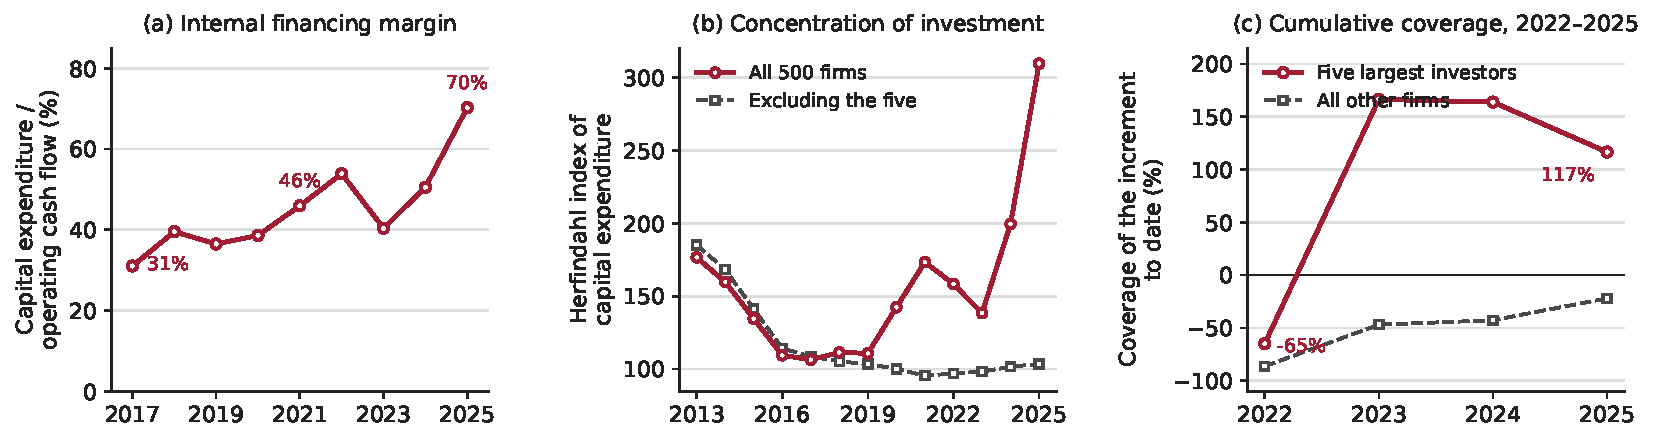
\includegraphics[width=\linewidth]{figures/Figure_1.pdf}
\caption{(a) Capital expenditure as a share of operating cash flow, the five largest incremental
investors, 2017--2025. (b) Herfindahl index of capital expenditure among the 500 largest U.S. public
companies by revenue, with and without those five firms. (c) Coverage of the increment cumulated
from the 2021 baseline through each year, on fixed membership: the five against the other 258
analysis firms.}
\label{fig:main}
\end{figure}

\section{Conclusion}
The financing of marginal projects need not define an investment boom in the aggregate. During the
AI buildout, internal cash coverage falls from 117\% at the five largest incremental investors to
$-61$\% across the remaining 213 firms. The gradient is specific to the current episode in our
comparison and is absent in the preceding two four-year windows, including the more concentrated
2018--2021 period.

This reconciles, rather than contradicts, the evidence on external finance, with project-finance
structures largely outside our sample. For the firms accounting for more than half of the increment,
incremental internal cash was in aggregate sufficient to cover their share of the boom, so the
headline size of the investment boom overstates the amount of incremental investment for which
incremental internal cash was insufficient. The result is time-specific: in 2025, capital
expenditure absorbed 70\% of the five firms' operating cash flow, versus 31\% in 2017, so internal
financing slack narrowed sharply over the sample.


\section*{CRediT authorship contribution statement}
\textbf{Samir Chincholikar:} Conceptualization, Methodology, Software, Formal analysis,
Writing -- original draft. \textbf{Robin Chawla:} Conceptualization, Validation, Writing --
review \& editing, Supervision.

\section*{Declaration of competing interest}
The authors declare that they have no known competing financial interests or personal
relationships that could have appeared to influence the work reported in this paper.

\section*{Funding}
This research did not receive any specific grant from funding agencies in the public,
commercial, or not-for-profit sectors.

\section*{Data availability}
The replication archive is deposited on Zenodo (\url{https://doi.org/10.5281/zenodo.22392416}) and contains the frozen source
files, the collection and analysis code, the machine-generated claims file against which every
reported number is checked, a SHA-256 manifest of every archived file, a one-command verification
script, and a companion document describing the archive in full.
Firm-level data were retrieved from the SEC's XBRL \emph{frames}
interface, one call per tag and year, at
\url{https://data.sec.gov/api/xbrl/frames/us-gaap/<tag>/USD/CY<year>.json}; 10-K text and
registrant classifications come from EDGAR and the submissions API
(\url{https://www.sec.gov/edgar/sec-api-documentation}). The tags unioned for each series,
including capital expenditure and operating cash flow, are listed in \texttt{code/engine.py}.
The deflator is Bureau of Labor Statistics series WPUFD41312, final demand--private capital
equipment, annual averages, retrieved with \texttt{code/collect\_deflator.py} from the BLS public
timeseries API. The \emph{frames} interface returns the
most recently filed value for each fact, so a later retrieval may differ where a filing or its
presentation has since changed; the frozen copies in the archive are the basis for every figure reported here.

\section*{Declaration of generative AI and AI-assisted technologies in the manuscript preparation process}
During the preparation of this work the authors used Claude (Anthropic) for code scaffolding, code
review, minor grammatical edits and readability improvements. The tool was not used to generate,
analyse or alter any datum, estimate, table or figure: all results are produced by the deposited
scripts from the frozen source files. After using this tool the authors reviewed and edited the
content as needed and take full responsibility for the content of the publication.

\begin{thebibliography}{99}
\bibitem{as} Ante, L., Saggu, A., 2025. Quantifying a firm's AI engagement: constructing objective, data-driven, AI stock indices using 10-K filings. Technological Forecasting and Social Change 212, 123965.
\bibitem{cg} Carvalho, V. M., Gabaix, X., 2013. The great diversification and its undoing. American Economic Review 103 (5), 1697--1727.
\bibitem{dgl} di Giovanni, J., Levchenko, A. A., Mejean, I., 2014. Firms, destinations, and aggregate fluctuations. Econometrica 82 (4), 1303--1340.
\bibitem{fhp} Fazzari, S. M., Hubbard, R. G., Petersen, B. C., 1988. Financing constraints and corporate investment. Brookings Papers on Economic Activity 1988 (1), 141--206.
\bibitem{gab} Gabaix, X., 2011. The granular origins of aggregate fluctuations. Econometrica 79 (3), 733--772.
\bibitem{ghw} Grullon, G., Hund, J., Weston, J. P., 2018. Concentrating on q and cash flow. Journal of Financial Intermediation 33, 1--15.
\bibitem{gp} Guti\'errez, G., Philippon, T., 2017. Investmentless growth: an empirical investigation. Brookings Papers on Economic Activity 2017 (2), 89--190.
\bibitem{hp} Hoberg, G., Phillips, G., 2016. Text-based network industries and endogenous product differentiation. Journal of Political Economy 124 (5), 1423--1465.
\bibitem{kz} Kaplan, S. N., Zingales, L., 1997. Do investment-cash flow sensitivities provide useful measures of financing constraints? Quarterly Journal of Economics 112 (1), 169--215.
\bibitem{lmcd} Loughran, T., McDonald, B., 2011. When is a liability not a liability? Textual analysis, dictionaries, and 10-Ks. Journal of Finance 66 (1), 35--65.
\bibitem{mm} Myers, S. C., Majluf, N. S., 1984. Corporate financing and investment decisions when firms have information that investors do not have. Journal of Financial Economics 13 (2), 187--221.
\bibitem{sta} Soto, P. E., Thieu, M., Allen, J. S., 2026. The AI buildout and the economy: publicly available data to assess AI's impact. FEDS Notes, 17 July.
\bibitem{vn} Van Nieuwerburgh, S., 2026. Financing the AI buildout. Working paper. \url{https://doi.org/10.2139/ssrn.6444363}.
\end{thebibliography}

\clearpage
\appendix
\setcounter{section}{0}
\renewcommand{\thesection}{Appendix~\Alph{section}}
\renewcommand{\thetable}{\Alph{section}\arabic{table}}\setcounter{table}{0}

\section{Supplementary evidence}\label{app:supp}

\subsection*{Table A1. AI attribution and AI-exposure robustness}
\begin{center}\footnotesize
\setlength{\tabcolsep}{4pt}\renewcommand{\arraystretch}{1.15}
\begin{tabularx}{\linewidth}{@{}l l X c@{}}
\toprule
\multicolumn{4}{@{}l}{\textit{Panel A. What the five firms' own filings say}}\\
Firm & Filing & Evidence & Capex--AI link \\
\midrule
Alphabet  & 10-K FY2025 & ``capital expenditures as we scale our technical infrastructure, in particular for AI'' & Explicit \\
Meta      & 10-K FY2025 & ``servers, data centers, and network infrastructure''; 2026 capital expenditure ``to support our AI efforts'' & Explicit \\
Microsoft & 10-K FY2026 & ``capital expenditures to support growth in our cloud offerings and our investments in AI training'' & Explicit \\
Oracle    & 10-K FY2026 & ``multi-year commitments for excess data center space and related capital expenditures''; not AI-explicit & Partial \\
Amazon    & 10-K FY2025 & cash capital expenditure ``primarily reflect[s] investments in technology infrastructure (the majority of which is to support AWS business growth)''; not AI-explicit & Partial \\
\bottomrule
\end{tabularx}
\end{center}
\begin{center}\footnotesize
\begin{tabular}{lrrr}
\toprule
\multicolumn{4}{@{}l}{\textit{Panel B. Coverage among firms ranked by AI intensity in their 10-K}}\\
& Firms & Share of increment (\%) & Coverage (\%) \\
\midrule
Top decile   & 26 & 41.9 & 126 \\
Top quintile & 52 & 43.5 & 131 \\
\bottomrule
\end{tabular}\end{center}
\noindent\footnotesize The five firms are selected mechanically from financial statements, not from AI disclosures. AI intensity is occurrences of a
pre-specified AI dictionary per 10{,}000 words of the firm's most recent 10-K, with top-decile and
top-quintile cutoffs of 2.25 and 1.35 fixed before any financing result was computed (Loughran and
McDonald, 2011; Hoberg and Phillips, 2016; Ante and Saggu, 2025). The five largest investors account
for 92.8\% of the top decile's incremental capital expenditure, so Panel B is a relabelled sample
rather than an independent one. Full dictionary, filing accession numbers and scoring code are in
the replication archive.\normalsize

\subsection*{Table A2. Data construction and validation}
\begin{center}\footnotesize
\begin{tabular}{@{}p{8.4cm}rl@{}}
\toprule
& Count & \\
\midrule
Observations reconciled (5 firms, 7 series, 2 years, where reported) & 49 & \\
Exact match to originally filed value & 48 & 98\% \\
Later filing uses gross-purchase presentation & 1 & Meta capital expenditure 2021 \\
Unexplained discrepancies & 0 & \\
\bottomrule
\end{tabular}\end{center}
\noindent\footnotesize Each constructed observation for the five focal firms is matched to a
10-K-reported value for the same fiscal period. The sole non-identical observation is Meta's 2021
capital expenditure. The FY2021 filing reports \$18.567bn, while the later FY2022 filing presents
\$18.690bn of gross purchases of property and equipment alongside \$123m of related proceeds. The
SEC interface returns the later gross-purchase presentation, which our series uses. Microsoft's fiscal year ends in June and Oracle's in May: Microsoft's 2025 observation covers July
2024 to June 2025 and Oracle's runs to May 2026, so the two windows fall either side of the December
endpoint used for the other three. We retain the SEC convention.
Capital expenditure and operating cash flow are unions of alternate tags; a single-tag
capital-expenditure series would omit Amazon and 454 other filers representing \$404 billion of 2025
spending. Deflator: BLS PPI WPUFD41312. All source files are frozen and
SHA-256 hashed, and every number is verified against a machine-generated claims file by an automated
build gate.\normalsize

\subsection*{Table A3. Firm-level and sectoral robustness}
\begin{center}\footnotesize
\begin{tabular}{lrrr}
\toprule
\multicolumn{4}{@{}l}{\textit{Panel A. The five largest incremental investors}}\\
Firm & $\Delta$Capex & $\Delta$OCF & Coverage \\
\midrule
Alphabet  & $96$ & $61$  & 63\% \\
Meta      & $81$ & $63$  & 77\% \\
Oracle    & $73$ & $46$  & 64\% \\
Microsoft & $67$ & $79$  & 118\% \\
Amazon    & $49$ & $177$ & 361\% \\
\addlinespace[3pt]
\multicolumn{4}{@{}l}{\textit{Leave-one-out: group coverage with the named firm omitted}}\\
Omitted firm & $\Delta$Capex & $\Delta$OCF & Coverage \\
\cmidrule{1-4}
Omit Alphabet & $270$ & $366$ & 135\% \\
Omit Meta     & $285$ & $364$ & 128\% \\
Omit Oracle   & $293$ & $380$ & 130\% \\
Omit Microsoft& $299$ & $347$ & 116\% \\
Omit Amazon   & $317$ & $249$ & 79\% \\
\bottomrule
\end{tabular}\end{center}
\begin{center}\footnotesize
\begin{tabular}{lrrr}
\toprule
& Firms & Share of tail (\%) & Coverage (\%) \\
\midrule
\multicolumn{4}{@{}l}{\textit{Panel B. Composition of the 213-firm tail}}\\
\quad Regulated and extractive & 25  & 19.9 & 122  \\
\quad Financial                & 25  & 7.1  & 298  \\
\quad All other                & 163 & 73.0 & -146 \\
\addlinespace[3pt]
\multicolumn{4}{@{}l}{\textit{Panel C. Coverage by rank, dropping regulated, extractive and financial firms}}\\
Rank group                     & Firms &      & Coverage (\%) \\
\cmidrule{1-4}
\quad Top 5                    & 5   &      & 117  \\
\quad Top 10                   & 10  &      & 97   \\
\quad Top 20                   & 20  &      & 90   \\
\quad Top 50                   & 50  &      & 80   \\
\quad Remaining                & 133 &      & -324 \\
\bottomrule
\end{tabular}\end{center}
\noindent\footnotesize Cumulative incremental flows, 2022--2025, baseline A (2021), billions of 2025 dollars. Coverage is
formed from unrounded flows, so it need not reproduce exactly from the rounded columns shown.
Panels B and C classify registrants by the SIC code in their own SEC filing: regulated and
extractive is oil and gas extraction, refining, rail, water and air transport, pipelines and
utilities; financial is banks and insurers, whose operating cash flow is not a comparable object.
Panel C drops both groups, leaving 183 firms.\normalsize

\end{document}
